% 来源：OEBPS/Text/Section0001_split_006.xhtml#sigil_toc_id_47

\BookChapter{34}
\section[第34章\q 约翰·博格：投资先锋]{第34章\\ 约翰·博格：投资先锋}

\begin{figure}[htbp]
\centering
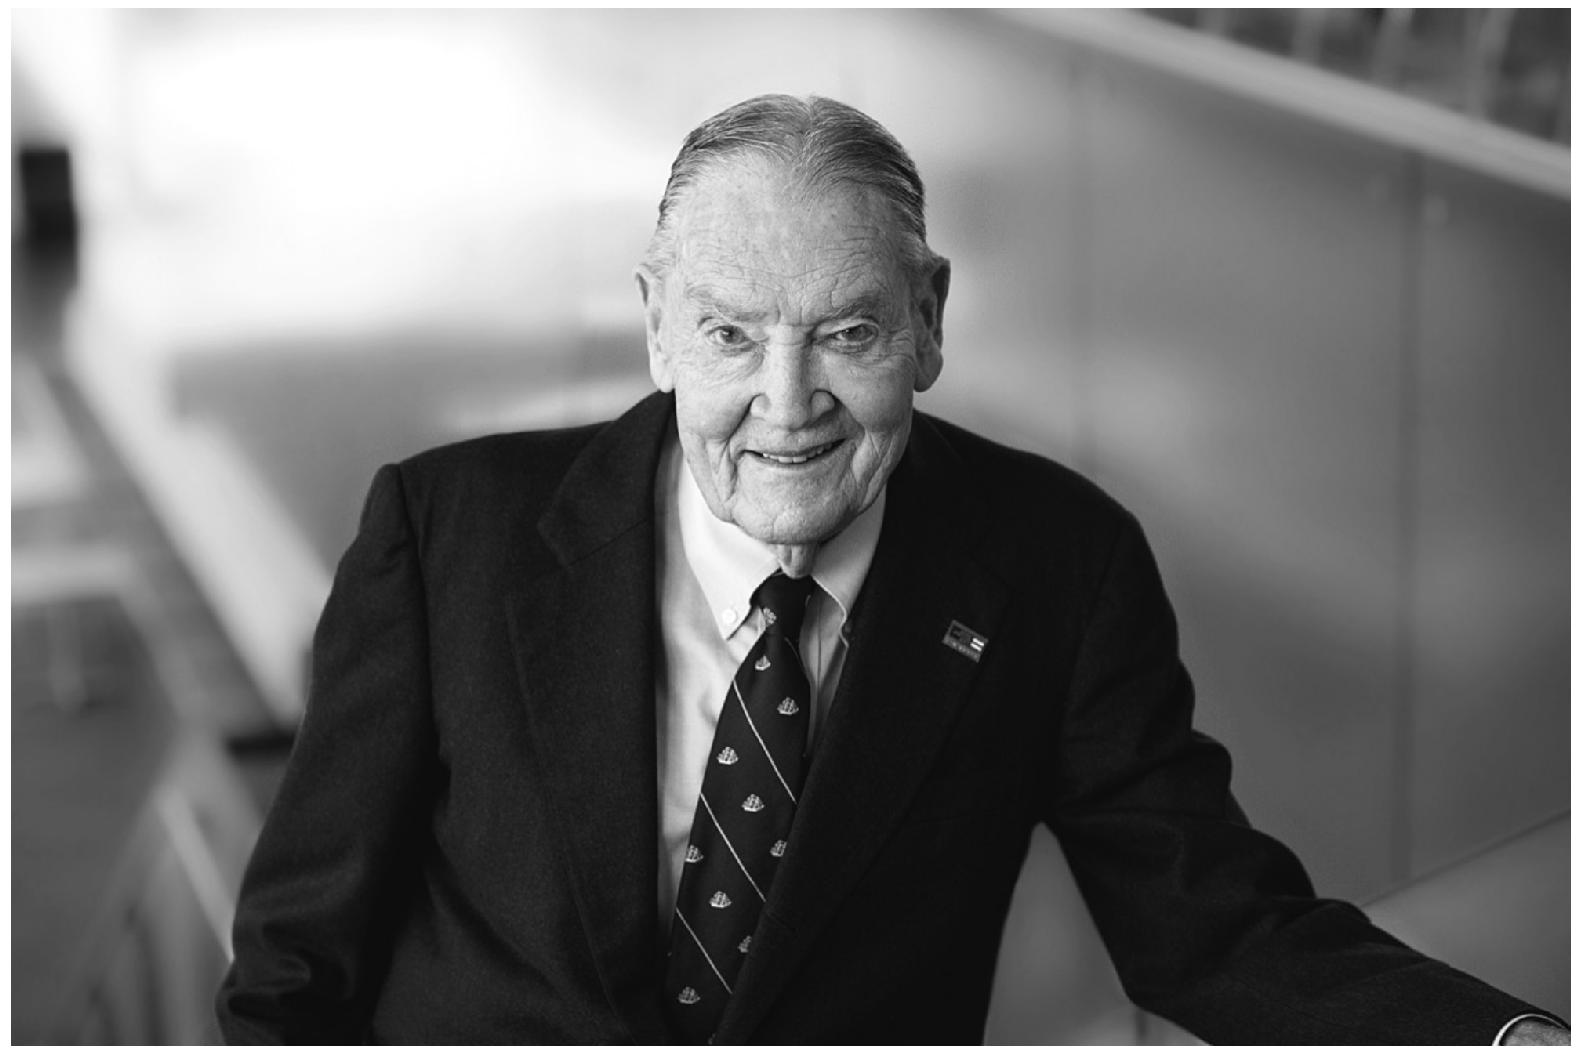
\includegraphics[width=0.56\linewidth,keepaspectratio]{image/约翰·博格肖像.jpg}
\caption*{约翰·博格}
\end{figure}

指数基金之父，先锋公司创始人和前任首席执行官

如果你没有读过约翰·博格的书，也没听过他在电视上一句废话都没有、全是干货的评论，那你就错过了一位美国国宝级投资大师。《财富》杂志将约翰·博格列为20世纪四大投资巨头之一。凭借突出的创造性和公民精神，有人把约翰·博格比作当代的本杰明·富兰克林。有人说，他对个人投资者做的贡献，超过美国历史上任何一个人。

他是如何做到如此巨大的成就，令人如此敬仰的？1974年，约翰·博格创立了先锋公司，那个时候指数基金还只是一个学术概念。但是约翰·博格愿意把整个公司押在指数基金上。指数基金是一个低成本低费用的公募基金，只单纯追踪整个股票市场的表现，时间一年年过去了，指数基金将会战胜绝大多数基金经理管理的主动型基金。为什么？投资者作为一个整体，绝对不可能战胜市场，因为投资者整体本身就是市场。基金行业的一些人知道来了一个破坏分子。首先，很多基金公司嘲笑博格的指数基金是“博格的傻瓜基金”，指数基金的竞争对手——那些主动管理型基金经理甚至说，指数基金这个想法太不像美国人的想法了，没有一点好胜心。

但是，约翰·博格根本不理会这些批评，继续坚持努力，把先锋公司打造成全世界最大的公募基金管理公司，管理规模达到2.86万亿美元。这个规模有多大？如果先锋公司是一个国家的话，那么这样的管理规模相当于英国的国内生产总值！现在，按照晨星评级公司的统计，美国指数基金在所有股票型公募基金的投资总额中占比超过1/3，也就是说，在美国，每3美元的股票公募基金，就有1美元是指数基金。

约翰·博格，1929年出生在美国新泽西州，恰好是美国经济大萧条开始的那一年。约翰·博格的家庭并不富裕，但是他聪明好学，后来考上了著名的普林斯顿大学，并且顺利毕业拿到了学位。约翰·博格在学校食堂打工，给其他同学做饭做菜，以赚取自己的学费和生活费。约翰·博格大学毕业写的论文主题就是公募基金，这预示着他以后要在公募基金行业开创一条新路。约翰·博格永远忘不了，有一年他暑假打工，当股票推销员朋友告诉他：“博格，我要告诉你，关于股市你需要知道的东西，都在这一句话里——没有人一无所知。”

1951年，约翰·博格大学毕业之后加入了惠灵顿基金管理公司，来到了费城。他不断地追求上进，步步高升，最后成了公司的总裁，在20世纪60年代中期那个热火朝天的大牛市里，约翰·博格把惠灵顿基金公司跟另外一家基金管理公司合并，希望这样能够促进公司业务的发展。“这是我一生最糟糕的错误。”他对我说。新来的合伙人把公司旗下的基金做得非常糟糕，然后利用他们在董事会的多数席位撤掉了约翰·博格的总裁职位。

突然遭受如此重大的危机，约翰·博格该如何应对？他没有接受失败，认输走人，而是把失败转化成他一生最大的成功，用创新改变了整个投资行业。由于公募基金的法律结构安排，博格还要继续负责惠灵顿公司的基金，但是与其管理公司分开经营运作，董事会成员也有所不同。约翰·博格留下来担任这些基金公司的董事长，但是他不被允许来管理这些基金的投资。“我怎么样才能做到不用成为基金经理，照样可以介入这些基金的投资管理？”他接受我的采访时说，“你已经知道答案了：创造出一种不用管理的基金。我们称之为指数基金。我给它起名叫先锋。一开始所有人都觉得我搞的指数基金完全是个笑话。”真不可思议，如果博格没有犯下那个大错的话，他就绝对不会创立先锋公司，亿万投资者也许就根本没有机会避免过度的基金收费，让他们的整体投资收益增加几十亿美元，甚至几百亿美元。

我和这位美国投资界的传奇人物面对面地坐在他的办公室里，在费城莫尔文的先锋公司园区里面，当时正是冬季，一场暴风雪席卷了美国东海岸。约翰·博格还是每天都上班。2000年，他卸任资深董事长之后，就开始负责先锋研究中心。一见面，85岁的约翰·博格跟我握手，力气很大，好像是一个只有他年龄一半的中年人。也许这是1996年移植心脏之后所赋予他的新的生命活力，让他可以继续他的投资改革运动，目标是给投资者公平的待遇。

我们交谈了4个小时，下面是经过编辑的访谈缩略版。

\begin{BookQuote}
\textbf{罗宾斯：}约翰·博格先生，请告诉我，您的驱动力从哪里来？
\end{BookQuote}

\begin{BookQuote}
\textbf{约翰·博格：}从我年轻时最早的记忆来，我必须工作。我9岁就开始工作了，在我们住的街区送报纸，我一直很喜欢送报纸。我是一个相当内向的人，长时间工作之后，就不会讲很多废话了。我这个人性格特别好胜，就是那种要跟人争斗一番的脾气，即使有时根本没有必要，这种好胜心弥补了我很多方面的不足。
\end{BookQuote}

\begin{BookQuote}
\textbf{罗宾斯：}您的职业生涯是从一家传统的公募基金管理公司开始起步的。
\end{BookQuote}

\begin{BookQuote}
\textbf{约翰·博格：}我那时还很年轻，还不够聪明睿智，我本来应该多从历史教训中吸取经验教训，依此采取行动。我当时还相信确实存在永久性的优秀基金经理，他们其实根本不存在。好的基金经理出现过又消失了。
\end{BookQuote}

\begin{BookQuote}
\textbf{罗宾斯：}为什么会这样？
\end{BookQuote}

\begin{BookQuote}
\textbf{约翰·博格：}其实投资业绩更多的是靠运气而不是靠能力。投资是95\%的运气加上5\%的能力，也许我说的还不太对，投资应该是98\%的运气加上2\%的能力。
\end{BookQuote}

\begin{BookQuote}
\textbf{罗宾斯：}每个主动管理型基金经理听了你这句话都会被气死。
\end{BookQuote}

\begin{BookQuote}
\textbf{约翰·博格：}我给你举个例子。要是你找来1024个人，聚到一个房间里，一起来比赛抛硬币。你告诉他们一起抛，连续抛上10次，那么这1024个人里面会有1个人连续10次正面朝上。你会说：“这个家伙真是太幸运了。”对不对？但是换成是在基金行业，你会说：“你真是个天才。”（哈哈大笑）你甚至可以把人换成大猩猩来抛硬币，结果完全一模一样。
\end{BookQuote}

\begin{BookQuote}
\textbf{罗宾斯：}您这样说的意思是不是说“一个聪明的人和一个优秀投资者之间有着巨大的差别”？
\end{BookQuote}

\begin{BookQuote}
\textbf{约翰·博格：}首先，投资者追求平均水平。我们先从这一点开始。非常简单。大多数个人投资者为得到平均水平的业绩付出了过高的成本。
\end{BookQuote}

\begin{BookQuote}
\textbf{罗宾斯：}这是怎么回事？
\end{BookQuote}

\begin{BookQuote}
\textbf{约翰·博格：}整体而言，你买主动管理型的基金平均要耗费你约2\%的成本（包括平均1.2\%的管理费，交易成本，现金拖累，销售手续费）。这意味着，如果市场平均业绩是7\%，那么扣掉付给基金公司2\%的费用之后，这些投资者只能得到5\%。（如果你买的是指数基金，成本只有0.05\%，这意味着你能得到6.95\%的收益率。）按照6.95\%的收益率，经过50年，你可以把1美元增值到30美元。但是，按照5\%的收益率，经过同样的50年，你只能把1美元增值到10美元，而不是30美元。这么大的收益差别意味着什么？这意味着，投资的本金100\%都是你付出的，投资的风险100\%都是你承担的，但是所有的投资收益里面，你能拿到手的只有30\%。看看股市的长期业绩，再看看主动管理型基金的长期业绩，你就会发现这个真实情况。很多人不愿意这么做，但是他们不得不学会这样做。
\end{BookQuote}

\begin{BookQuote}
\textbf{罗宾斯：}他们没有搞明白成本的复利效应和费用的复利效应。
\end{BookQuote}

\begin{BookQuote}
\textbf{约翰·博格：}这些人应该真正搞明白他们为什么要买股票。买股票的真正目的是要得到股利即现金分红，是为了得到盈利增长。事实上，从长期来看，股票市场的收益一半来自股利即现金分红。所有基金的费用支出也都是从这里出的。所以你好好想一想，托尼，我告诉你，平均每只基金的股利收益率是2\%，平均每只股票基金的费率是1.2\%，羊毛出在羊身上，基金的管理费都是从基金分到的现金分红里扣掉的，所以你拿到手的股利收益率只剩下0.8\%，基金公司从你的股利收益率里面拿走了一半来付给它们自己作为基金的管理费！整个基金行业向基金持有人收取的费用占属于投资者股利收入的60\%，有的时候是100\%，有的时候甚至超过100\%。现在你能明白为什么我对基金行业如此痛心，它吃掉投资人的收益实在太多了。
\end{BookQuote}

\begin{BookQuote}
\textbf{罗宾斯：}但是还有1亿人投资主动管理型公募基金。这些人怎么可能这样任人宰割？
\end{BookQuote}

\begin{BookQuote}
\textbf{约翰·博格：}绝对不要低估市场营销的力量。回到2000年，我们来看看，那些在《金钱》杂志上打广告的公募基金，平均年度业绩为41\%，这些基金有很多，甚至可能是大多数，现在都不存在了。基金投资者预期，他们选择的聪明基金经理，会永远聪明下去，但是根本不会有这种事。基金投资者心里的预期是，这个聪明的基金经理上一年创造出来20\%的年收益率，将来能够持续很多年创造出来20\%的收益率。这种想法太荒谬可笑了。这不可能发生，这绝对不可能发生。
\end{BookQuote}

\begin{BookQuote}
\textbf{罗宾斯：}先锋公司的经营管理，只是为了让公司的基金持有人受益，实际上先锋公司是由基金持有人持股的公司。您支持统一受托人标准了？
\end{BookQuote}

\begin{BookQuote}
\textbf{约翰·博格：}我是这个要求的提出者。也许我是第一个提出这个要求的人。投资公司研究所（公募基金行业的游说组织）说：“我们并不需要制定一个联邦式的受托责任的标准，我们就是受托人。”那么，既然如此，第一点，为什么他们还要反对这件事？这是一个很有趣的问题。
\end{BookQuote}

但是，第二点，他们不明白，我们有受托责任冲突，一个上市公司，比如贝莱德集团，有两个受托责任：一个是对贝莱德集团旗下公募基金的股东有受托责任，责任是让股东赚到最多的钱；另外一个受托责任是对贝莱德集团的股票持有人，也就是公众持有人有受托责任，要尽可能赚到最多的钱，责任是要让这些基金持有人的收益最大化。因此，贝莱德集团的首席执行官劳伦斯·芬克就陷入了终极的两难处境。要让贝莱德集团的基金持有人的收益最大化，他就必须降低收费，但是要让贝莱德集团的股东收益最大化，他就必须提高收费。你不可能同时做到这两点，既提高收费，又降低收益，你只能选择一条路。贝莱德集团努力想要同时做到这两点。结果是现在这家公司给股东赚的钱比以前任何时候都要多。

\begin{BookQuote}
\textbf{罗宾斯：}这太讽刺了。
\end{BookQuote}

\begin{BookQuote}
\textbf{约翰·博格：}美国是个伟大的国家，不然怎么会有这种事？
\end{BookQuote}

\begin{BookQuote}
\textbf{罗宾斯：}按照您的看法，下一个最急迫也最具挑战的事情是什么？
\end{BookQuote}

\begin{BookQuote}
\textbf{约翰·博格：}我认为，美国上市公司会继续成长，记住，股票市场是一个衍生物，它是我们上市公司创造的价值的衍生物。美国上市公司现在为股东赚钱，将来会继续为股东赚钱，也许可能会赚得少一点儿。但是，美国上市公司规模会变得越来越大，而且生产效率会越来越高。所以它们会继续增长，也许比我们习惯的速度要稍微慢一点儿，但是还会是一个健康的增长速度。
\end{BookQuote}

\begin{BookQuote}
\textbf{罗宾斯：}主要是因为消费会下降，这是基于人口统计资料，或者是因为我们借的钱太多了，我们买房花的钱还没有还清。
\end{BookQuote}

\begin{BookQuote}
\textbf{约翰·博格：}我们还得继续去杠杆，我们美国的借债太多了。公司这方面其实没有太多的借债，美国公司方面的负债率并不高，资产负债表相当不错。但是，美国政府，包括联邦政府、州政府和地方政府，负债率都太高了，我们必须做出行动来解决这些债务问题。
\end{BookQuote}

其中的一个风险是个大问题，就是现在美联储有4万亿美元的存款准备金，和正常水平相比多出3万亿美元，这3万亿美元差不多都是最近5\textasciitilde{}6年量化宽松多出来的，必须消化掉。谁都搞不清楚这件事是怎么发生的。但是每个人都知道这件事迟早会发生。

\begin{BookQuote}
\textbf{罗宾斯：}我们是不是要小心会再发生金融危机？
\end{BookQuote}

\begin{BookQuote}
\textbf{约翰·博格：}如果你觉得你不是像一般投资者那样思考，而是像那些有大视野的人那样思考，绝对不要丧失你对历史的感觉。不要认为历史不会重演。正如马克·吐温所说的：“历史可能不会重复，但是历史的节奏会重复。”所以，我们将来确实有可能再发生一次严重的全球金融危机，甚至是全球经济大萧条，但是全球经济大萧条的概率有多大？我说可能是1/1000的概率。但这并不是1/10的概率，所以我并不认为全球大萧条可能会发生，但要是有人说全球经济大萧条绝对不可能发生，那就错了。
\end{BookQuote}

\begin{BookQuote}
\textbf{罗宾斯：}这样说肯定是没有好好研究历史。
\end{BookQuote}

\begin{BookQuote}
\textbf{约翰·博格：}是的。这件事基本上只要你用常识就能想明白。不要让一时的潮流和一时的风尚冲昏你的头脑，也不要被市场一时的盘旋冲昏你的头脑，不管是股市还是债市。
\end{BookQuote}

\begin{BookQuote}
\textbf{罗宾斯：}您在投资行业干了64年，您经历过各种各样的市场波动起伏，您是怎么在投资中抽离人的感情因素的呢？
\end{BookQuote}

\begin{BookQuote}
\textbf{约翰·博格：}没有人能够做到，包括我在内。我只是努力在投资时尽量减少感情因素。人们会说，要是股市跌了一半，你会有什么感觉？我说，老实说，我感觉非常痛苦。我的心都揪得紧紧的。那么我能做点儿什么减轻一些痛苦？我会找出来一两本讲“坚持到底”的书，再读一遍。
\end{BookQuote}

\begin{BookQuote}
\textbf{罗宾斯：}如果您不能把任何一分钱传给你的子孙后代，但是您可以传给他们一些投资基本原则，您会告诉他们什么？
\end{BookQuote}

\begin{BookQuote}
\textbf{约翰·博格：}我会告诉他们三个投资基本原则：第一个原则是，注意你投资的是什么类型的资产。你选择你的资产配置，要跟你的风险承受度和你的目标保持一致。第二个原则是，分散投资，你一定要用低成本的指数基金来做分散投资，有很多基金都是成本很高的。我们不要忘了这一点。第三个原则是，不要交易。什么都不要做，一直拿着你的指数基金，放在那里！不管发生什么事，一直持有不动。你要是想让自己更容易抵抗住下跌的恐惧那么继续持有不动，你可以在做资产配置时，在你原来觉得合适的债券配置比例的基础上，再稍微多加上一点点。
\end{BookQuote}

\begin{BookQuote}
\textbf{罗宾斯：}您对投资者还有什么其他建议？
\end{BookQuote}

\begin{BookQuote}
\textbf{约翰·博格：}别看《华尔街日报》！别看电视上播出的那些财经节目！开个玩笑。我上过很多次美国全国广播公司的电视节目，多次接受采访，我一直很奇怪，为什么他们一次又一次地问我。吉姆·克莱默的节目，我看上40\textasciitilde{}50秒就受不了了。那些股票电视节目，都是在大喊大叫地让你买这个股票，卖那个股票。这只会让你偏离投资的本质，只会让你分心。我们浪费了太多时间，浪费了太多能量，关注那些与投资相关的东西，其实你知道结果会是什么样的。你只能得到市场平均业绩，即和市场指数相同的业绩，有时多一些，有时少一些。大多数时候只会比市场平均水平少一些。所以，为什么你还要花这么多时间整天交易标准普尔500指数，就像早期的外汇交易基金市场营销大战建议的那样？只要一直持有标准普尔500指数，你就可以轻松地拿到平均业绩。
\end{BookQuote}

那些一直持有指数基金的人，赚的最多的不是钱，而是时间，是生活。不做频繁交易，不天天折腾，给你节省大量的时间精力，让你更多地享受生活。带孩子去公园玩，带家人出去吃顿晚餐。如果这些都做不了，你也可以读一本好书。

\begin{BookQuote}
\textbf{罗宾斯：}钱对您意味着什么？
\end{BookQuote}

\begin{BookQuote}
\textbf{约翰·博格：}我不把钱看成目标，而是把钱看作达到目标的手段，有一个很精彩的故事，讲的是两位作家库尔特·冯内士特和约瑟夫·海勒。他俩在谢尔特岛一个聚会上碰到了，于是一起喝酒。库尔特·冯内士特看看约瑟夫·海勒，对他说：“你看那个人，我们今天聚会的东道主，就在那里。你知道吗，这家伙今天赚了1亿美元。他一天赚的钱比你那本书《第22条军规》所有的版税加在一起还要多。”约瑟夫·海勒回过头来看看库尔特·冯内士特，然后说：“那也没什么，因为我有些东西，他再有钱也永远不会有。这就够了。”
\end{BookQuote}

我留给孩子的财富足够他们干自己想干的事，但是并不够养着他们什么事都不用干。我经常对他们说：“有的时候，我真希望你们能有我小时候那样的成长经历，你们就能拥有我拥有的所有优势了。”我的孩子听后的第一反应是：“像你那样长大，你说的应该是劣势吧？”“不，孩子，我说的是优势。穷得只能勉强生活，努力工作，努力打拼，闯出一条自己的路。”

\begin{BookQuote}
\textbf{罗宾斯：}投资大众花了好多年才接受指数基金的概念，现在指数基金像风暴一样席卷整个基金行业，规模占比超过1/3。您当年创造第一只指数基金的时候，您怎么感觉指数基金这条路是对的？
\end{BookQuote}

\begin{BookQuote}
\textbf{约翰·博格：}人们说，你肯定非常骄傲。看看你创造的指数基金现在规模多么庞大。我告诉他们，它还有很大的发展空间，我觉得，到了将来某一天，我才能说可以了，现在还没有到那一天。我记得索福克勒斯说过：“我们必须等到晚上才能欣赏到白天的光辉灿烂。”我的晚上还没有到来。
\end{BookQuote}

你知道的，我要坦白地说，我很早以前就遭遇了死亡。做心脏移植手术之前，我有过8次心脏病发作。我的心跳都停止了，我根本没法活下去。但是我后来做了心脏移植，我继续活下来了，这实在是太不可思议了。我没有花太多时间来考虑这件事，但是我认识到，我正亲眼见证指数基金大胜，投资者现在青睐指数基金，这真的是一场革命性的变化，这一点毋庸置疑。指数基金正在改变证券行业。现在证券公司赚的佣金和基金公司赚的管理费比以前少了好多。我并不确定我能够完全理解这件事，但是我想，要是我死了，我就看不到指数基金的巨大胜利。

\begin{BookQuote}
\textbf{罗宾斯：}顺便问一下，您会退休吗？
\end{BookQuote}

\begin{BookQuote}
\textbf{约翰·博格：}可能这件事更多的是上帝说了算，而不是我自己说了算。能活着，我很享受，我很享受我的生活和我的工作，我的使命是给投资者带来公平的待遇，我以此为乐。
\end{BookQuote}

\subsection{约翰·博格的投资组合核心原则}

1.资产配置要与你的风险承受能力和你的目标保持一致。

2.通过低成本指数基金进行分散投资。

3.你的债券基金配置比例要跟你的年龄一样大。这是一个“大致”的基准。

约翰·博格现在80多岁，他的投资组合中40\%投资在债券上。但是一个非常年轻的人可以把资产百分之百地投资在股票上。

所以，我的整个投资组合，包括我的个人账户和退休金账户，60\%左右的资产投资在股票上，大部分都是先锋公司的股票指数基金，其余的40\%被分成两部分，一部分投资在先锋公司的全债券市场指数基金，另一部分投资在免费（市政）债券基金，我的市政债券是这样分散投资的，2/3投资先锋公司的中期免税债券基金，另外1/3投资先锋公司的有限期限免税债券基金（有限意味着在短期和中期之间。期限长一点儿，收益会多一点儿）。

我希望我不需要从我的含税投资组合里面提取现金。我的免税投资组合，是有相当不错的免税收益率的，有3\%左右，按照我的税级来说，这相当于税前5\%的税率。我不需要比这更高的收益率了。能拿到这么多，我已经很开心了。

当然我也有一点儿担心市政债券市场的稳健性，但是我相信，有我们先锋公司的一流分析师，这两只市政债券基金应该会做得不错。在我的递延纳税投资组合里，这也是我最大的一部分资产，我的债券资产大部分都配置在先锋公司全债券市场指数基金上。这只债券基金持有的债券包括长期、中期、短期债券，还包括国债、抵押贷款、公司债券。

我对我的投资组合整体收益率非常满意。尽管2008年这一组合下跌了17\%，很惨，但是那一年标准普尔500指数下跌了37\%，比我的投资组合净值跌幅高出200\%以上。我的投资组合收益率一直是正的，平均每年约10\%。我很高兴，我只是一直持有，坚持到底，结果安然地度过了金融危机大熊市。
